\section{Performance} \label{sec:perform}

The Start Counter was installed in Hall-D just prior to the Fall 2014 \gx{} commissioning run.  It was not until the Spring 2015 commissioning run that enough statistics were obtained with an $\mathrm{LH_{2}}$ target to perform reliable calibrations.  With the aforementioned data set the procedures to calibrate the detector, as discussed in Sec.~\ref{sec:calib}, and measure it's performance were developed and deployed.

As was discussed in previous sections, the geometry of the ST nose section results in an increase of the light output as the scintillation source moves towards the downstream end.  While investigating FADC250 data under nominal beam conditions, this phenomenon was immediately observed through both the pulse amplitude and pulse integral data. Figure~\ref{fig:pippvszint} illustrates that, similar to the bench measurements, the light output increases exponentially as the scintillation source moves towards the downstream end.
% WB one spectrum would probly be enought Amplitude or Pulse integral (here both look the same)
% EP They are in-fact the same.  They are place holders at the moment.  It will be a game-time decision as to whether or not we include both.
	\begin{figure}[!htb]
		\centering
		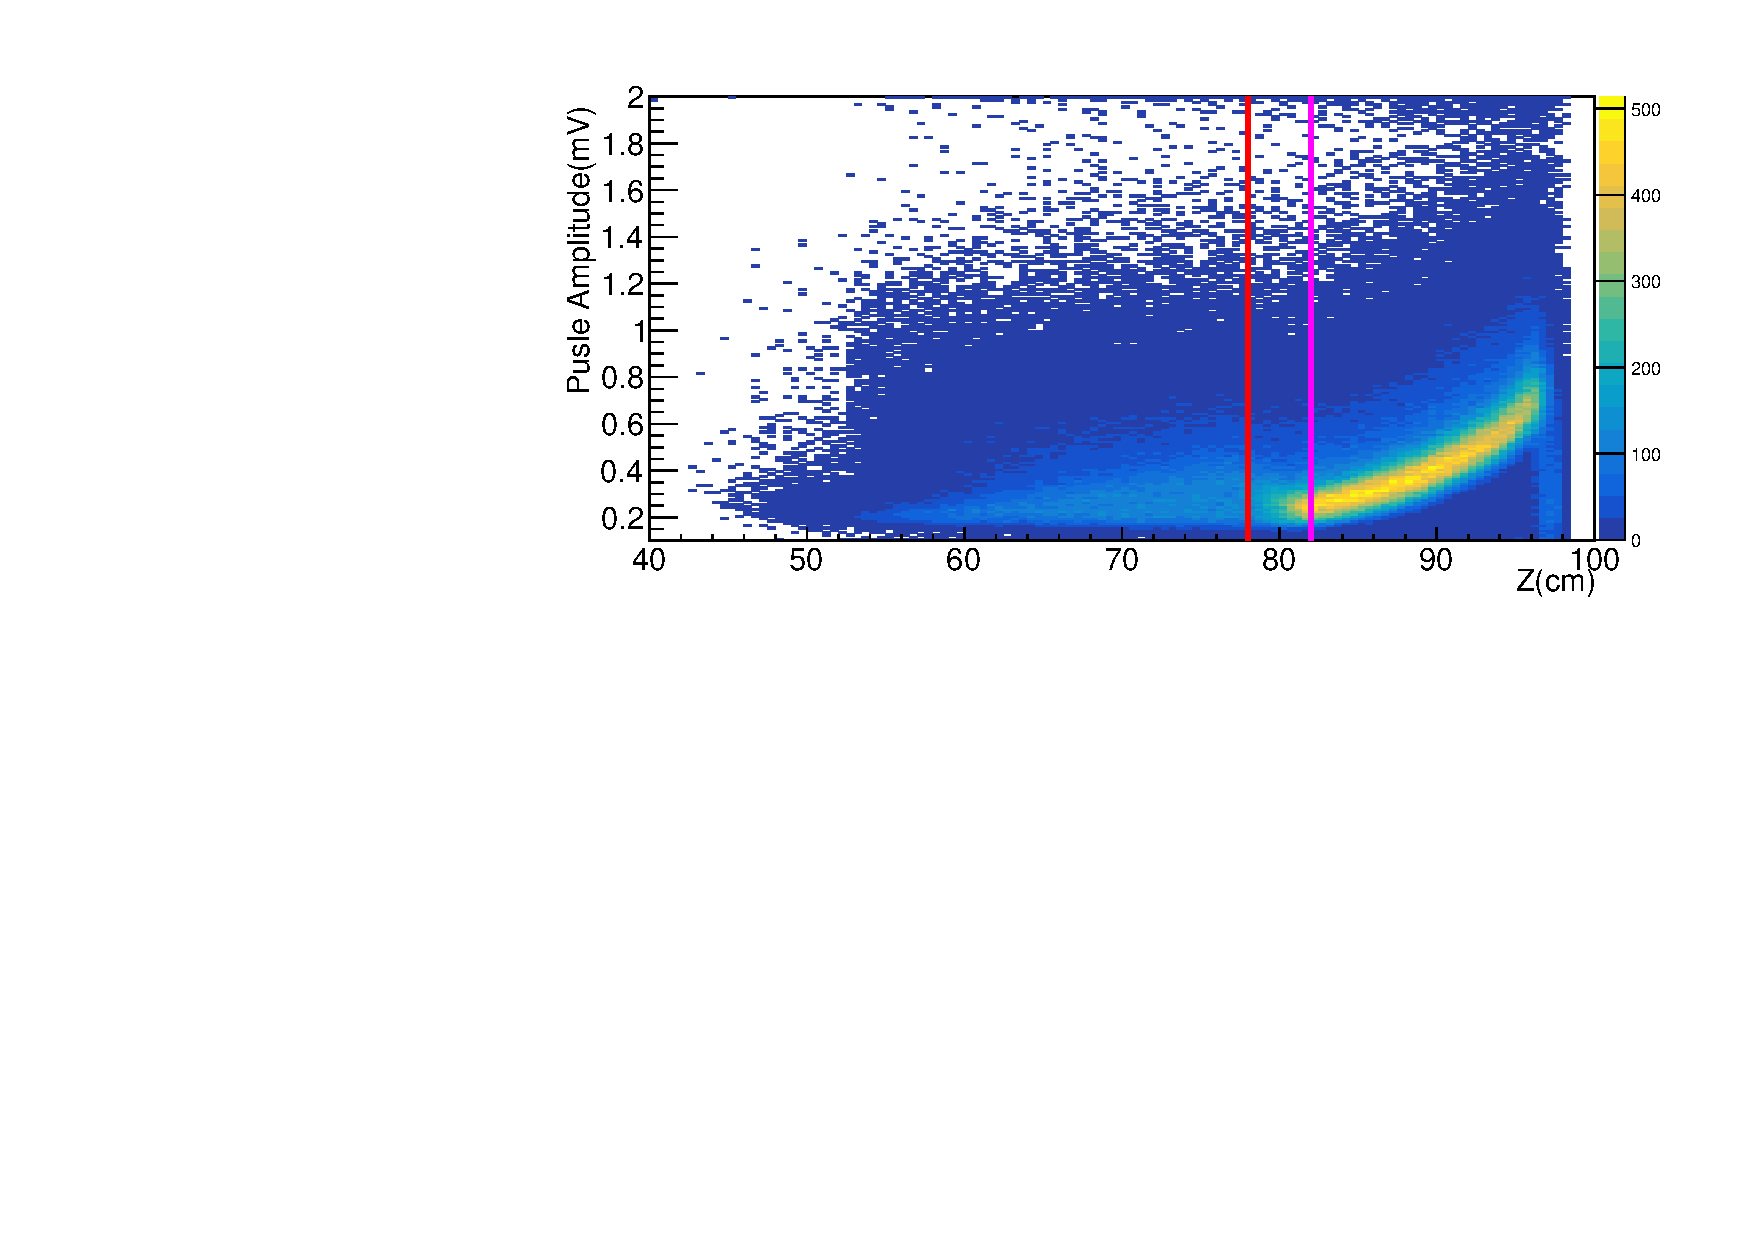
\includegraphics[width=1.0\columnwidth]{performance/figs/PA_Z}
		\caption{Typical FADC250 pulse amplitude spectra versus the $z$-component of charged tracks intersecting the ST for an individual ST sector. The vertical lines from left to right indicate the end of the straight section, and the start of the tapered nose section respectively.}
		\label{fig:pippvszint}
	\end{figure}
This feature of the ST geometry is quite advantageous since the majority of the charged tracks produced under the nominal \gx{} beam conditions intersect the ST in the nose region and therefore have the largest light amount of light collected by the SiPM's at the upstream end.

Once the proper attenuation corrections discussed in Sec.~\ref{sec:calib_ac} were applied to the data, the PID capabilities of the ST were greatly enhanced.  Figure ~\ref{fig:dEdx_vs_p_corr} illustrates the PID capability of charged tracks intersecting the ST.  
	\begin{figure}[!htb]
		\centering
		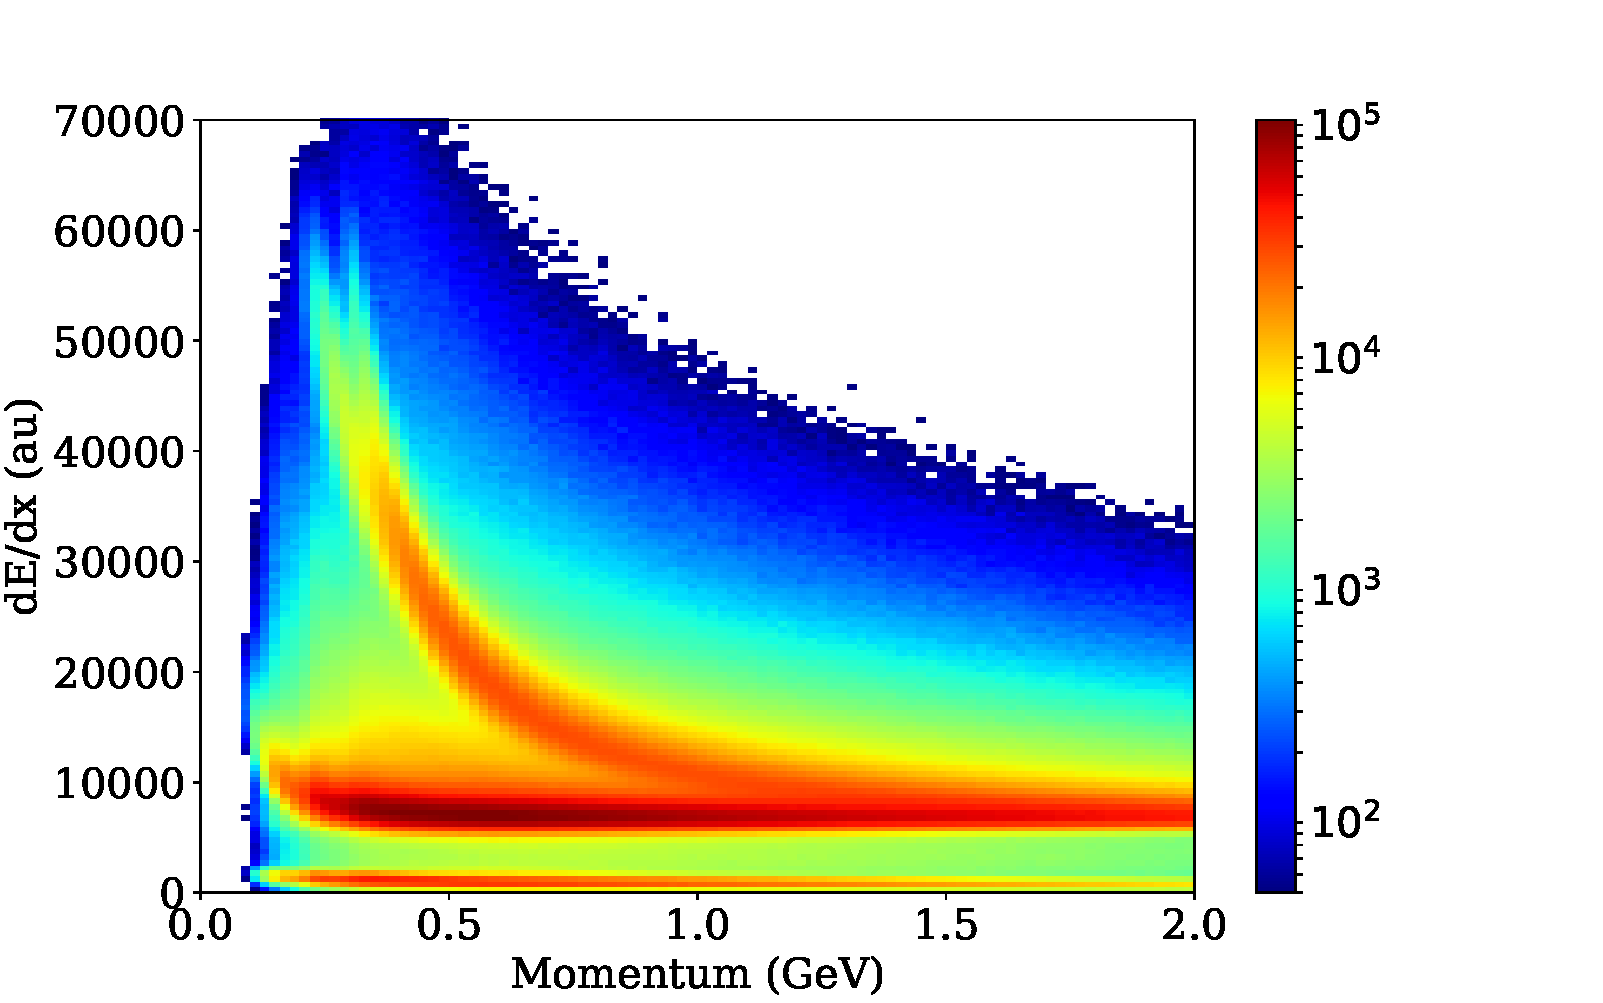
\includegraphics[width=1.0\columnwidth]{performance/figs/Att_corr}
		\caption{Corrected $dE/dx\ vs.\ p$ distribution for tracks matched to the Start Counter.  The ``banana band'' corresponds to protons while the horizontal band corresponds to charged electrons, pions, and kaons.  It is clear that pion/proton separation is achievable for tracks with $p < 1.1\ \mathrm{GeV/c}$.}
		\label{fig:dEdx_vs_p_corr}
	\end{figure}  
The reliable separation of protons and other hadrons occurs for charged tracks with $p < 1.1\ \mathrm{GeV/c}$ which is a factor two improvement relative to the uncalibrated data.  The PID capabilities of the ST are particularly advantageous for successfully identifying low momentum and backwards going protons which do not propagate into the central drift chamber surrounding the ST.

After the time-walk and propagation time corrections discussed in Sec.~\ref{sec:calib_tw} \& \ref{sec:calib_ptc} were complete, it was then possible to utilize the ST to measure times associated with charged track vertices for tracks matched to it.  The vertex time is defined to be the time in which a polarized Bremsstrahlung photon interacted with the $\mathrm{LH_{2}}$ target and produced a charged track and is given by Eq.~\ref{eq:st_vertex_time}.  Measuring the ST vertex time relative to the beam bunch vertex time provided by the accelerator is the most robust way to determine the ST ability to successfully identify the beam buckets associated with a particular event.  An identical charged track selection process, as outlined in Sec.~\ref{sec:calib_ptc}, was utilized so that the time resolution of tracks matched to the ST could be measured.  

The resulting distribution in the time difference of ST vertex time $(T^{ST}_{vertex})$ and the measured time the beam bunch arrived at the track vertex $(T^{BB}_{vertex})$ provides a measure of the ST time resolution and is seen in Fig. \ref{fig:st_time_res}.
	\begin{figure}[!htb]
		\centering
		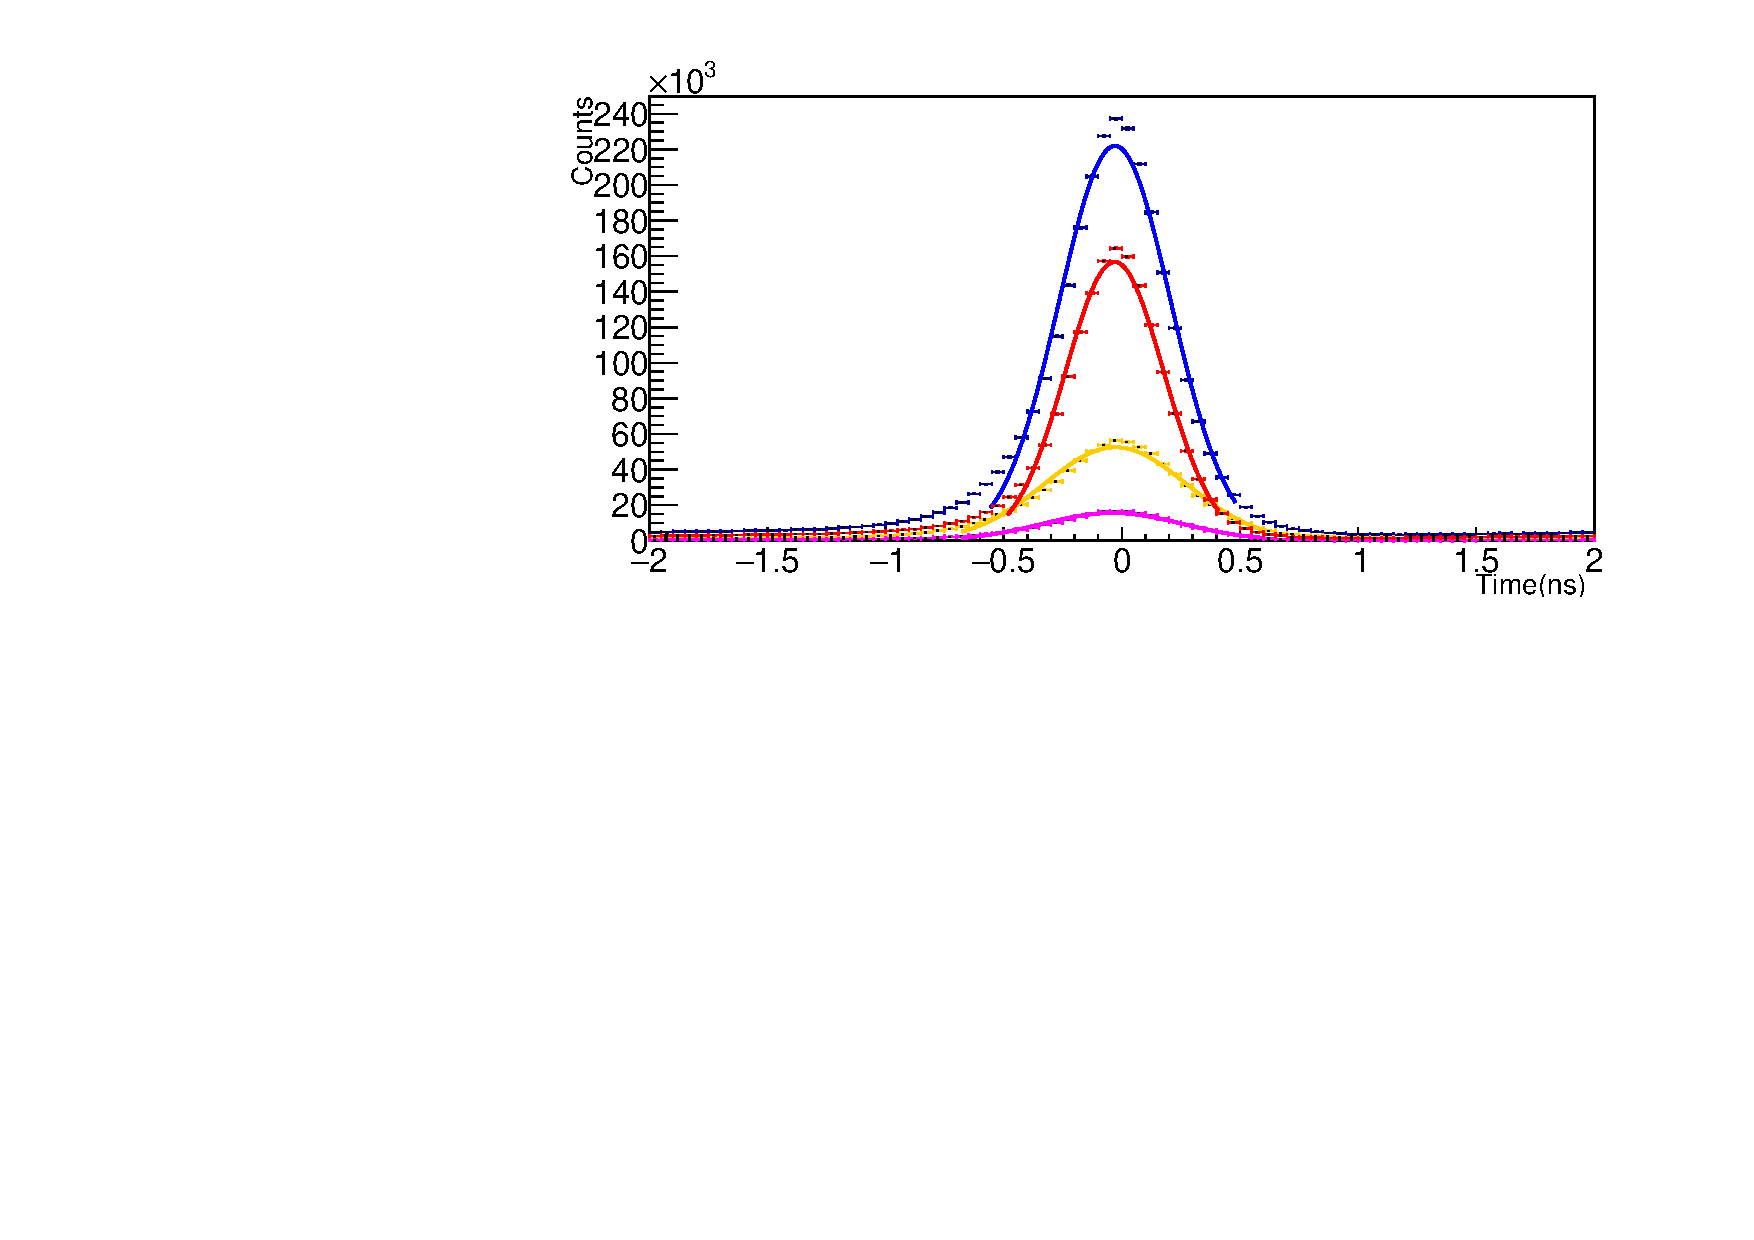
\includegraphics[width=1.08\linewidth]{performance/figs/TR_15}
		\caption{Typical Start Counter time - RF time resolution distribution.  The x-axis is the time difference between $T^{ST}_{vertex}$ and $T^{BB}_{vertex}$. The orange histogram is the resolution in the straight section. The magenta and red histograms correspond to the resolution in the bend and nose sections respectively. The blue histogram is a sum of the three sections and corresponds to the resolution along the entire length of the paddle.}
		\label{fig:st_time_res}
	\end{figure}
% EP This plot is not needed, the results should be summarized in a table.
%	\begin{figure}[!htb]
%		\centering
%		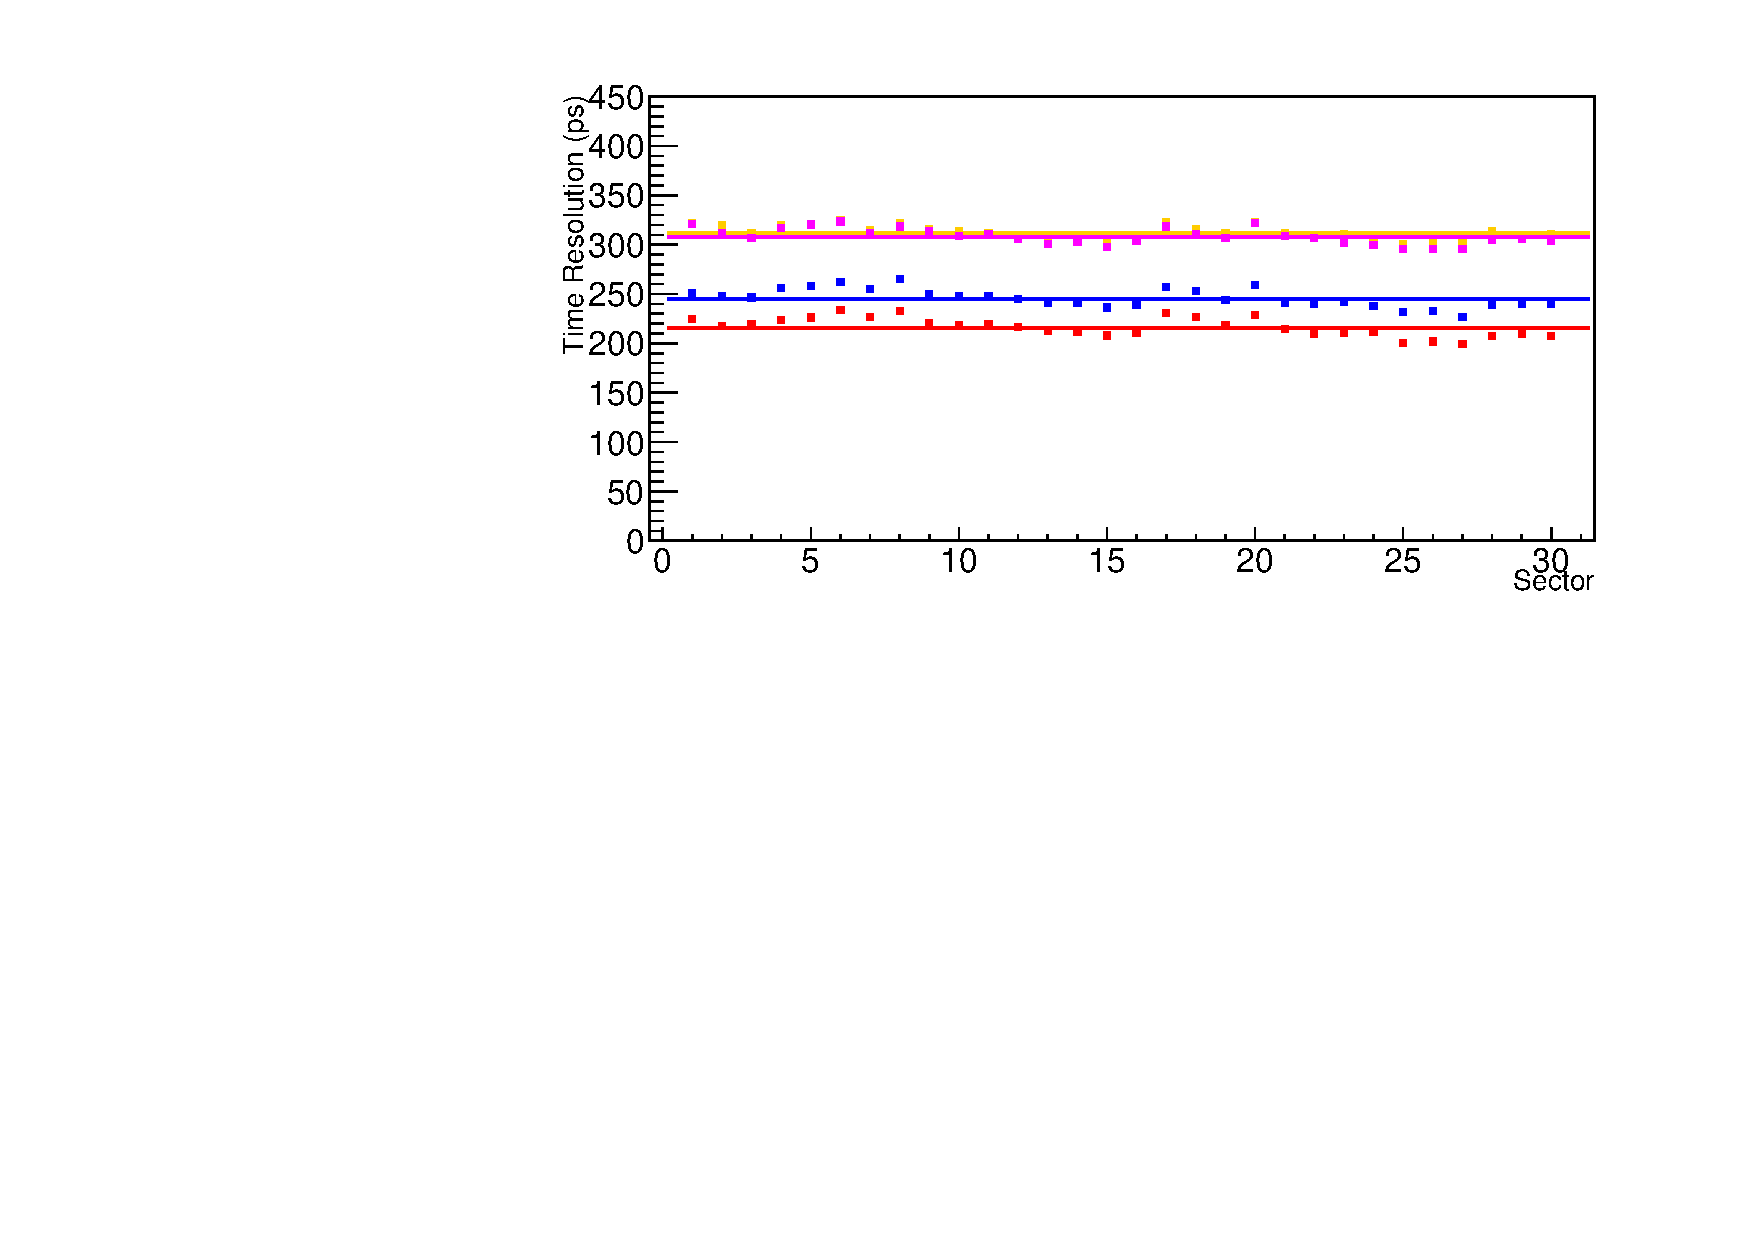
\includegraphics[width=1.08\columnwidth]{performance/figs/TR_All}
%		\caption{ST time resolutions as a function of sector number (Blue line). Orange and magenta lines are the average time resolution for the straight and bend sections respectively. The nose section resolution is greatly enhanced due to the exponential increase in light output (red).}
%		\label{fig:timeresallinset}
%	\end{figure}	
Gaussian fits were then applied to the data seen in Fig.~\ref{fig:st_time_res} in order to quantify the time resolution performance of the ST paddles.

The aforementioned fits were carried out for each of the ST sectors with $\sigma$ and its associated error being calculated.  Then a weighted average of the 30 $\sigma$'s were calculated so that the ST could have its time resolution characterized in its entirety.  The same procedure was also conducted for the three individual geometrical sections.  Table~\ref{tab:time_res_section} details the weighted average time resolution of all the ST sectors in the different geometrical regions.
	\begin{table}[htbp]
		\centering
		\begin{tabular}{|c|c|c|c|c|}
			\hline  \textbf{Section} & $\mathbf{\sigma_{all}}$ & $\mathbf{\sigma_{straight}}$ & $\mathbf{\sigma_{bend}}$ & $\mathbf{\sigma_{nose}}$ \\ 
			\hline $\mathbf{\sigma_{avg}}$ & 245 ps & 314 ps & 309 ps & 216 ps \\ 
			\hline 
		\end{tabular}
		\caption{Average time resolutions by section. Shown is the average of all 30 ST sectors by independent geometrical regions.}
		\label{tab:time_res_section}
	\end{table}

The ST exhibited uniformity in time resolution among all sectors of the ST. The data also indicates that the average time resolution of 245~ps is well below the design resolution of 350~ps.  It is clear from Table~\ref{tab:time_res_section} that what is observed is that measurements made with beam data exhibit the same phenomenon of substantial improvement in light collection, and thus time resolution, as light is produced further downstream in the nose region.

When these time resolution measurements were conducted with data collected in Spring 2017, approximately 3 years had elapsed since the paddles were first tested on the bench at FIU.  Prior experience with degrading scintillators indicates that degradation in time resolution will be visible in a matter of weeks.  However, after 3 years no degradation has been observed and the ST is still performing well below design resolution.